\newpage
\subsection{Technologie Diagramme}
 Hier werden die Zusammenhänge der Technologien in Form von verschiedenen Diagrammen vorgestellt.

\subsubsection{UML Komponentendiagramme}
Hier werden die UML Verteilungsdiagramme von der Server- und Client-Seite dargestellt.

\subsubsection{UML Komponentendiagramm: Client}
Hier wird fer UML-Komponentendiagramm Client dargestellt.

\begin{figure}[H]
    \centering
    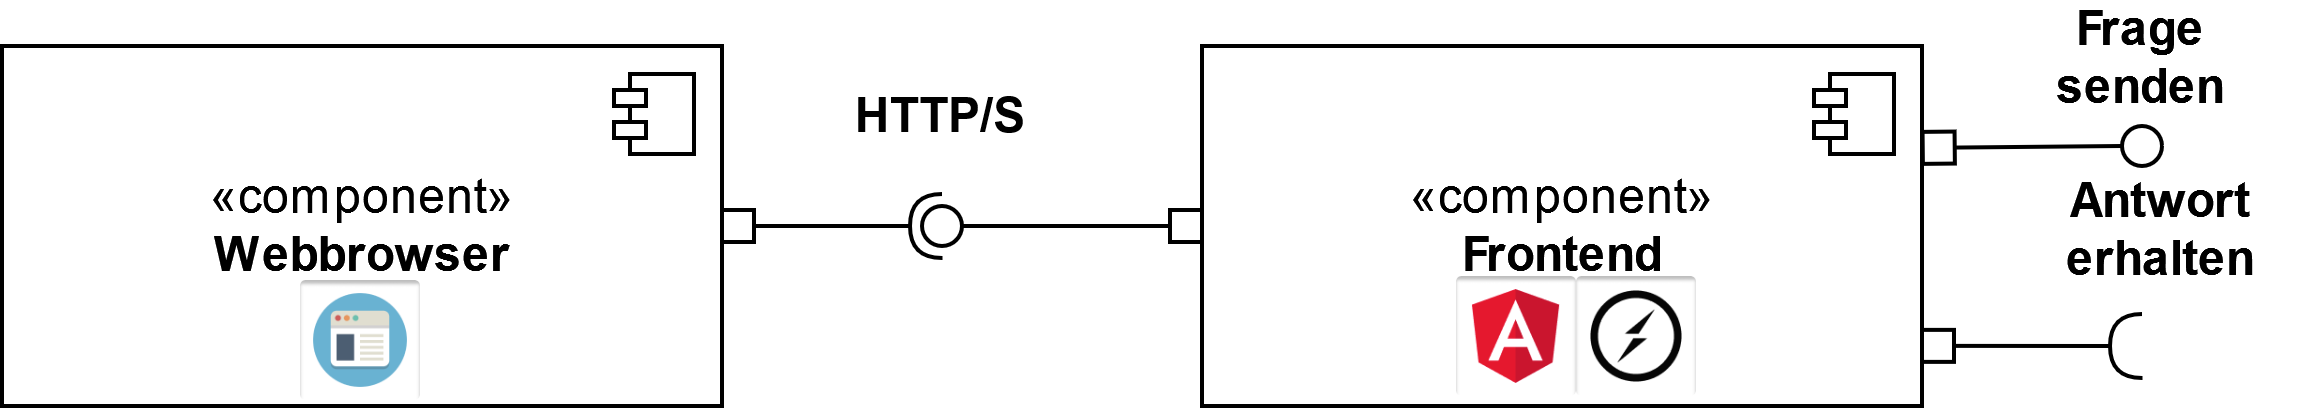
\includegraphics[width=1.0\textwidth]{bilder/technologien/UML_Komponentendiagramm_Client.png}
    \caption{UML Komponentendiagramm Client}
    \label{fig:UML_Komponentendiagramm_Client}
    \end{figure}
\noindent In der Abbildung \ref{fig:UML_Komponentendiagramm_Client} sieht man, dass der Webbrowser und das Fronted auf der Client Seite.
Das Fronted wird mit Angular entwickelt. Das besitzt aber selber auch einen node.js Server.
Per Socket.io Client wird dann eine Verbindung zwischen den Backend produziert. Per HTTP/S
wird eine Vebindung zwischen Webbrowseerund dem Fronted entwickelt. Das Frontend component 
sendet eine Frage und erhält anschließend eine Antwort vom Backend.   

\newpage

\subsubsection{UML Komponentendiagramm: Server}
Hier wird der UML-Komponentendiagramm Server dargestellt.

\begin{figure}[H]
    \centering
    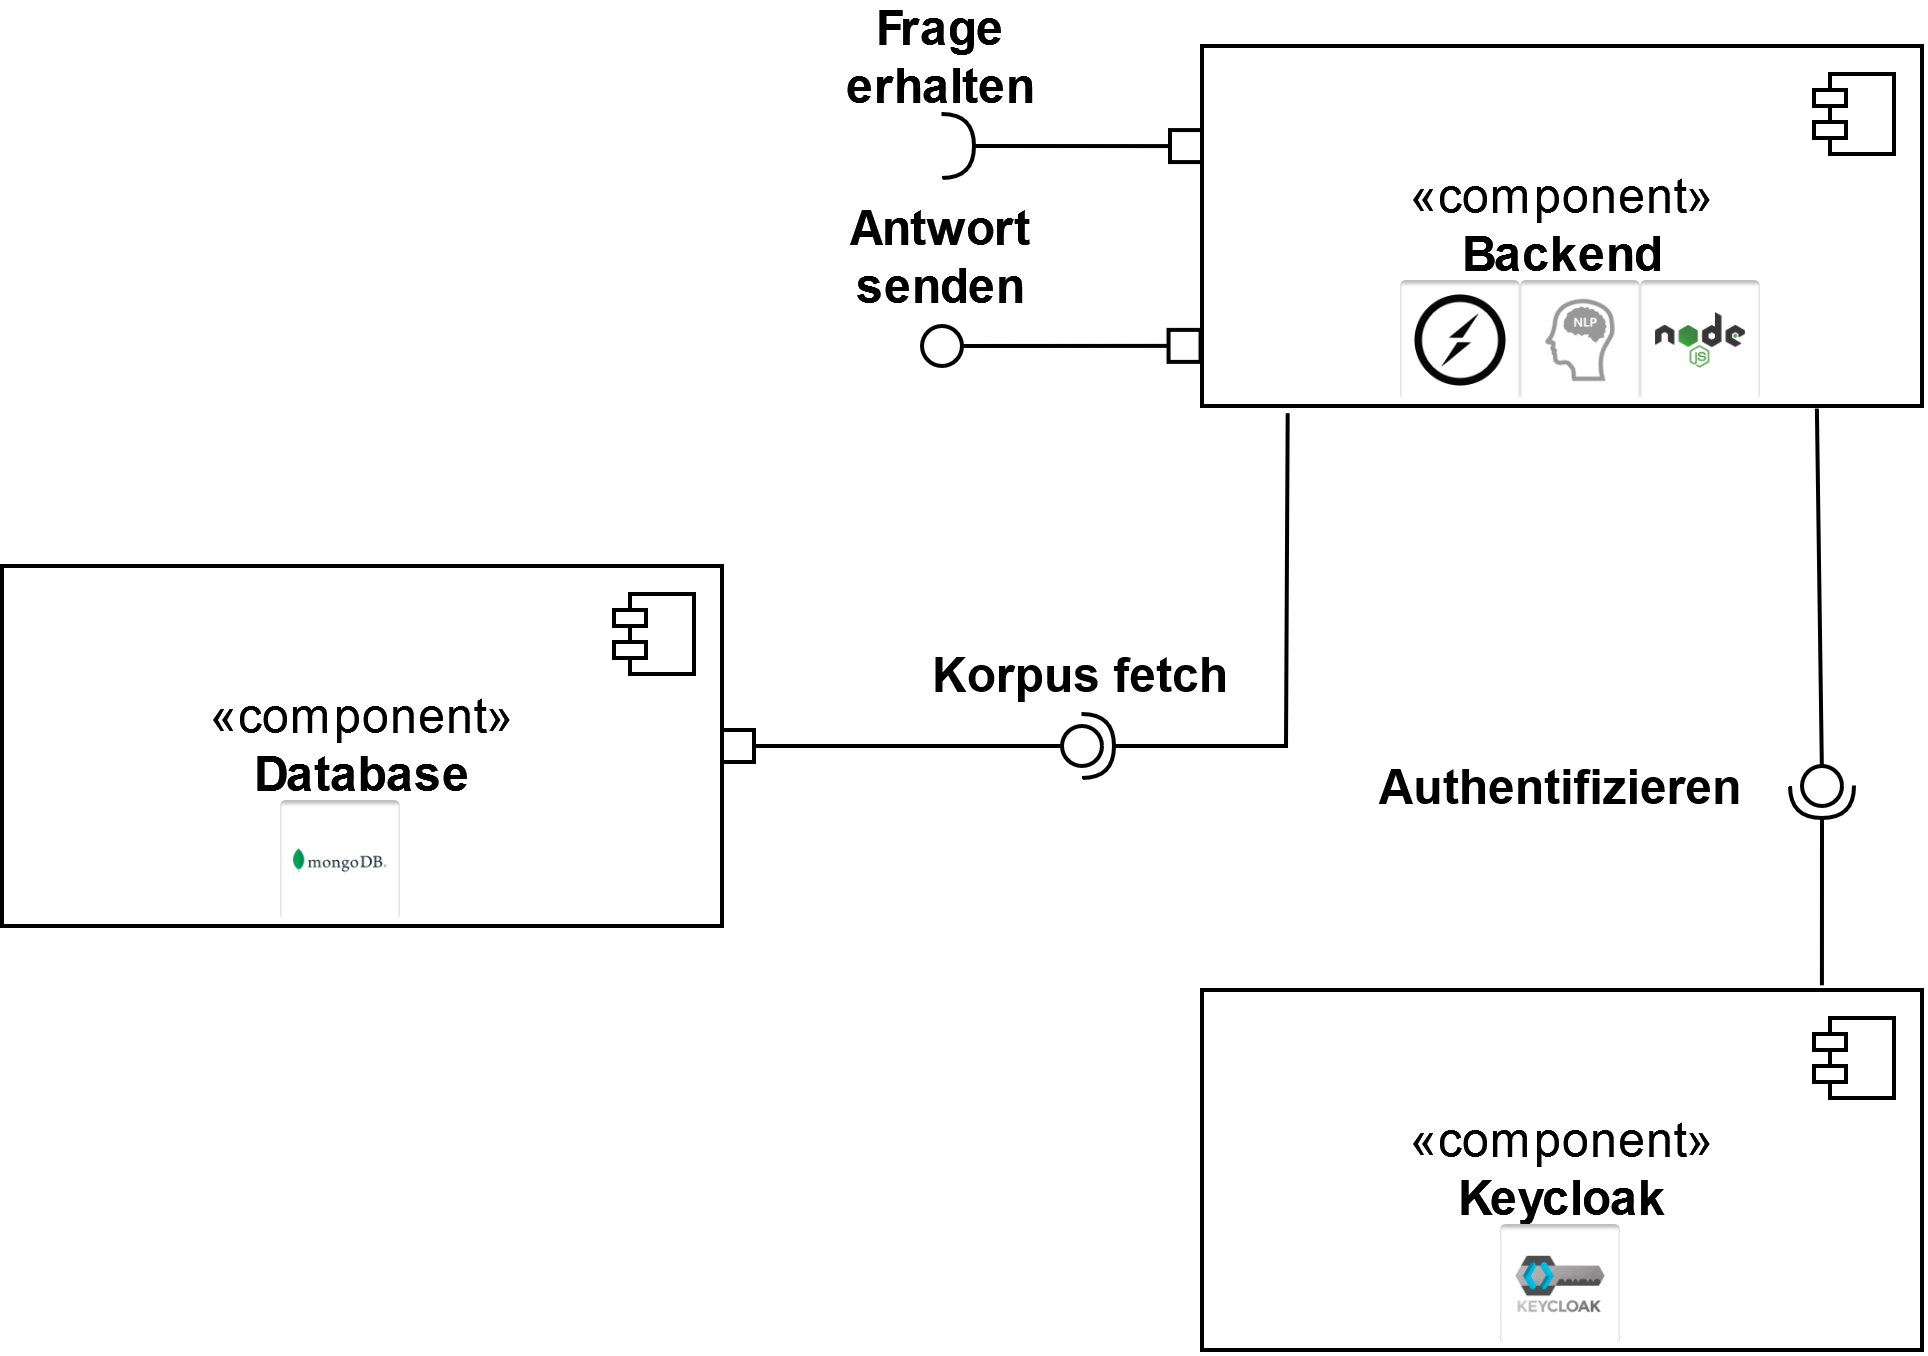
\includegraphics[width=1.0\textwidth]{bilder/technologien/UML_Komponentendiagramm_Server.png}
    \caption{UML Komponentendiagramm Server}
    \label{fig:UML_Komponentendiagramm_Server}
    \end{figure}
\noindent In der Server-Seite befindet sich das Backend, die Datenbank und das KeyCloak.
Im Backend befindet sich der Socket.io Server, NLP und ein node.js Server.
Das Backend erhält die Frage vom Fronted und schickt daraufhin eine Antwort mit Hilfe des Socket.io Servers zurück.
Von der Datenbank wird der Korpus, and das Backend, vermittelt. KeyCloak dient zur Authentifizierung und
hat ebenfalls einen node.js Server. 

\newpage

\subsubsection{UML Komponentendiagramm}
Hier sieht man die ganze Darstellung von dem Komponentendiagramm mit Server- und Client-Seite.
\begin{figure}[H]
    \centering
    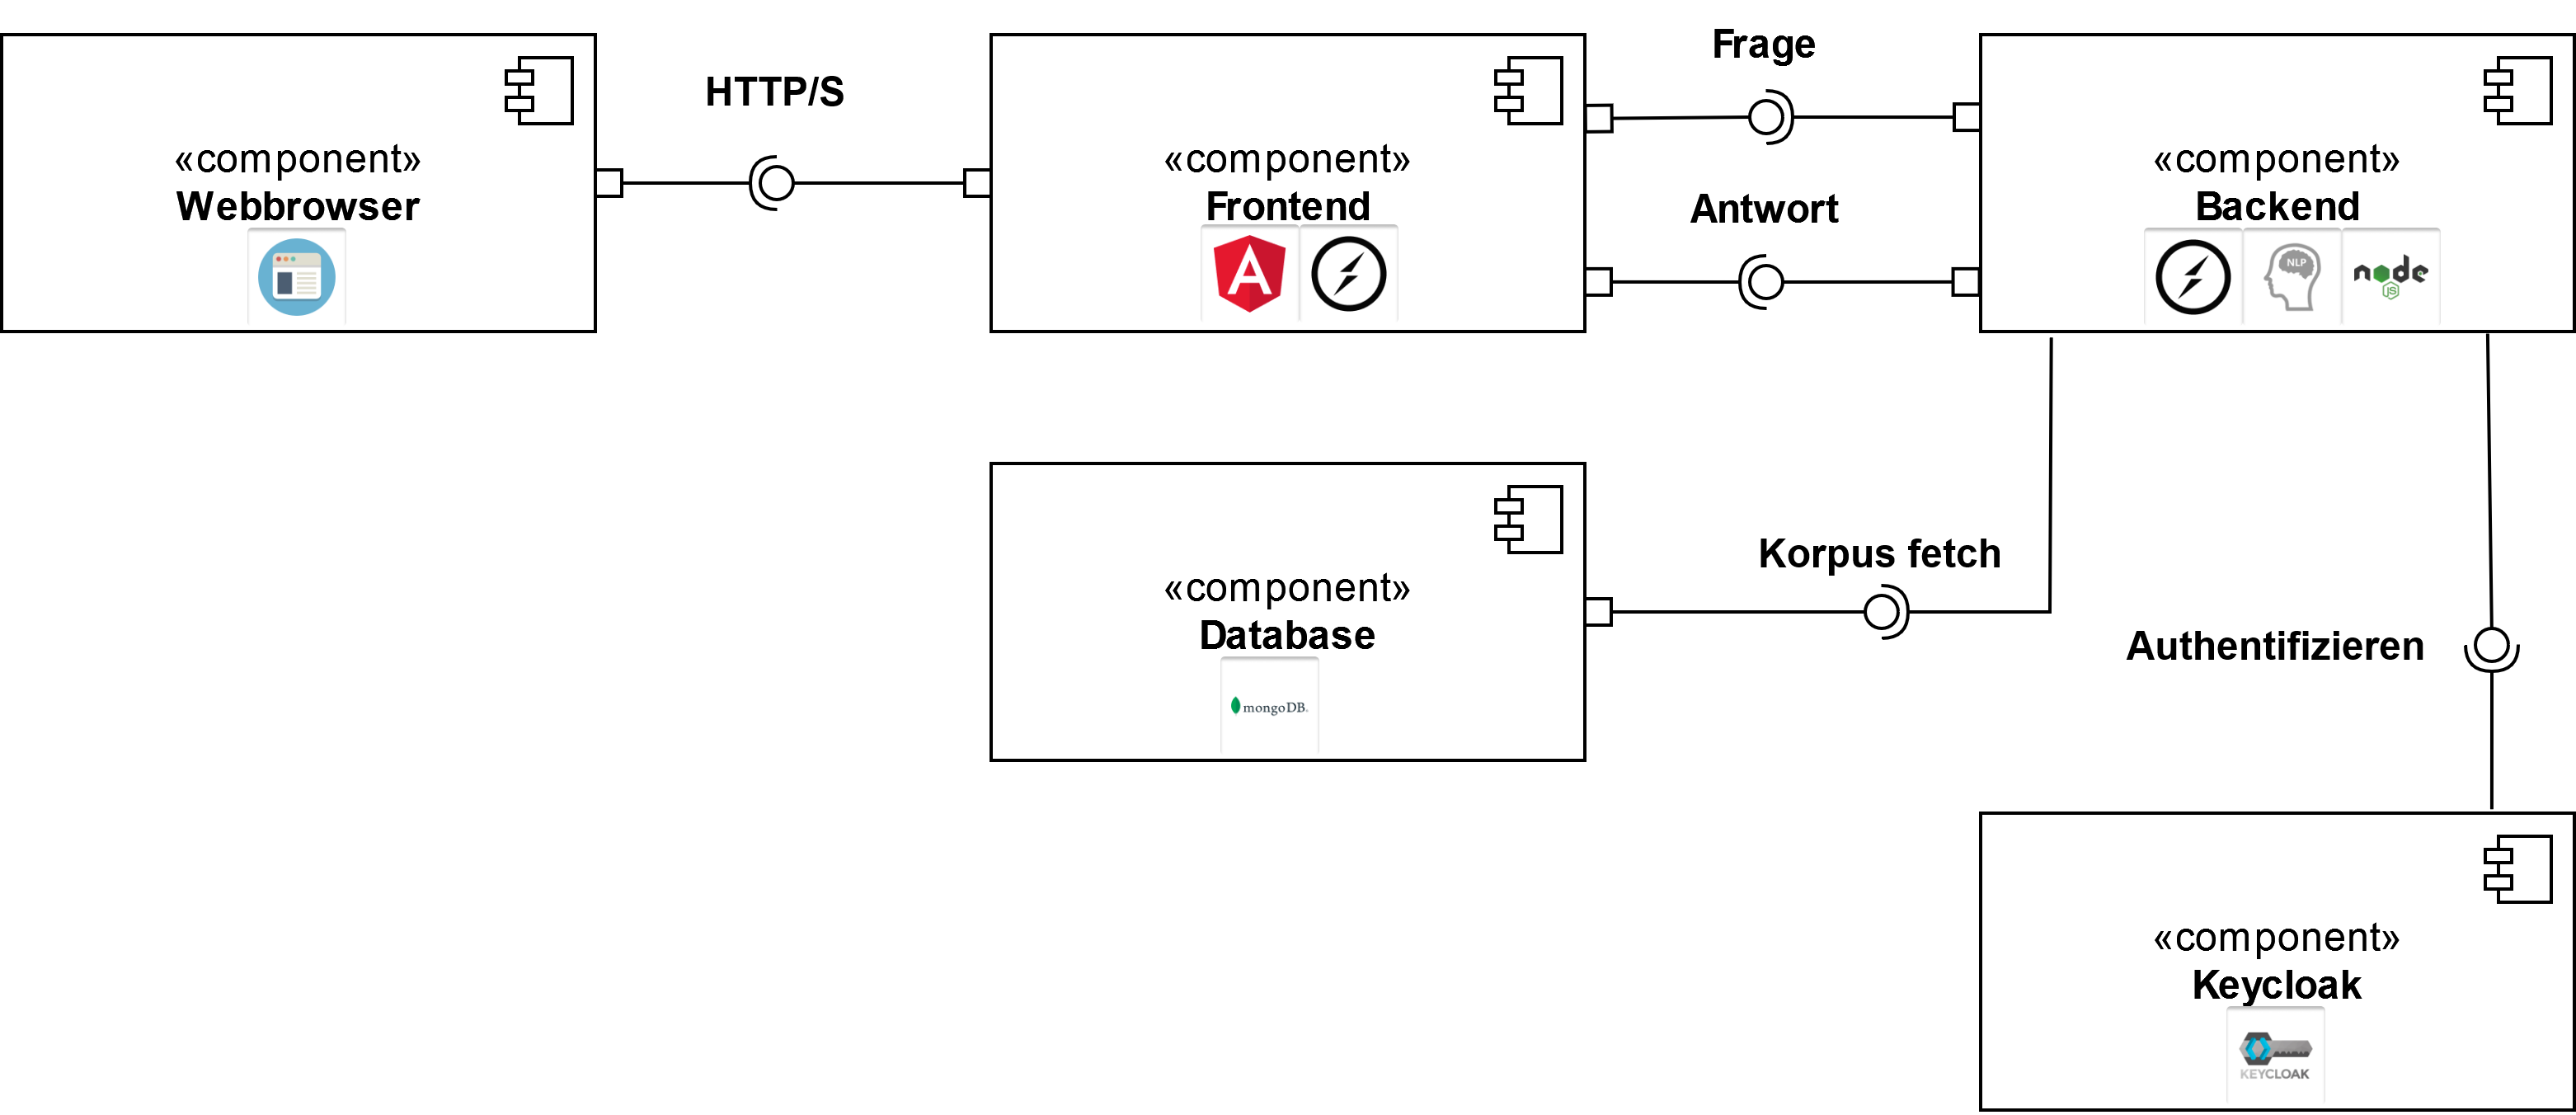
\includegraphics[width=1.0\textwidth]{bilder/technologien/UML_Komponentendiagramm.png}
    \caption{UML Komponentendiagramm}
    \label{fig:UML_Komponentendiagramm}
    \end{figure}
\noindent In dieser Abbildung \ref{fig:UML_Komponentendiagramm} sieht man die Client- und Server-Seite. 
Als Austausch zwischen Fronted und Backend haben wir eine Frage und eine Anwort dargestellt.
Des weiteren besitzt das Frontend, das Backend und KeyCloak einen node.js Server.

\newpage

\subsubsection{UML Verteilungsdiagramm}
Hier sieht man die ganze Darstellung unseres Verteilungsdiagramms
\begin{figure}[H]
\centering
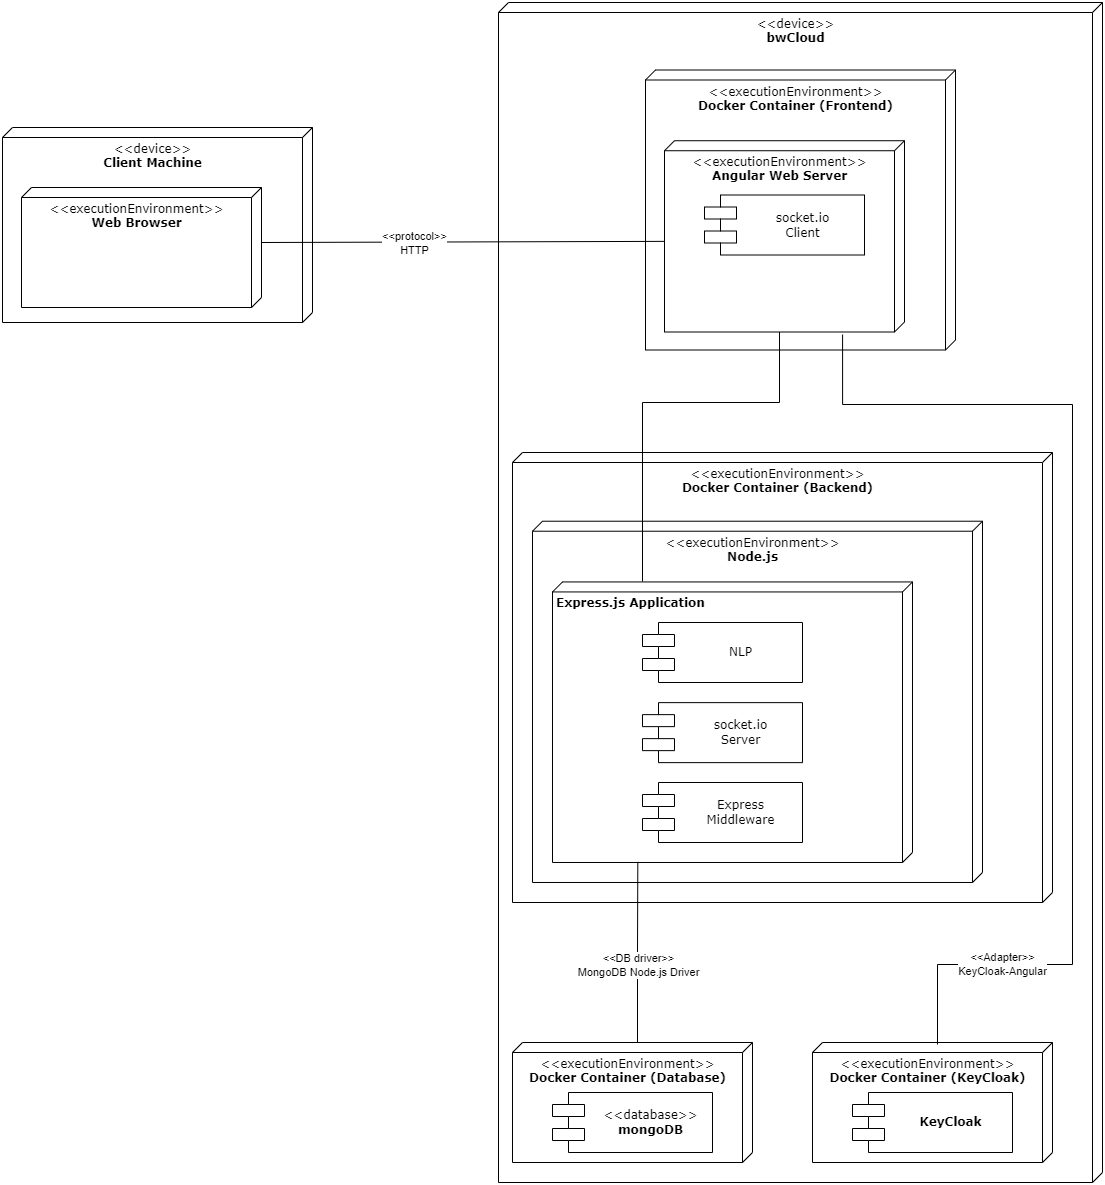
\includegraphics[width=1.0\textwidth]{bilder/technologien/UML_Verteilunsgdiagramm.png}
\caption{UML Verteilungsdiagramm}
\label{fig:UML_Verteilungsdiagramm}
\end{figure}
\noindent In unserem Verteilungsdiagramm kann man sehen, 
wie die verschiedenen Technologien verschachtelt und wie sie miteinander verbunden sind.
Außerdem kann man sehen, was wir in unsere einzelnen Dockercontainer hineinlegen.